
\documentclass{aa}  

\usepackage{graphicx}
%%%%%%%%%%%%%%%%%%%%%%%%%%%%%%%%%%%%%%%%
\usepackage{txfonts}
%%%%%%%%%%%%%%%%%%%%%%%%%%%%%%%%%%%%%%%%
%\usepackage[options]{hyperref}
% To add links in your PDF file, use the package "hyperref"
% with options according to your LaTeX or PDFLaTeX drivers.
%
\begin{document} 


   \title{The data center for the X-ray Imaging Spectrometer/Telescope STIX}

   \subtitle{}

   \author{H. Xiao
          \inst{1}
          \and 
          Shane Maloney 
          \inst{2}
          \and 
          Ewan Dickson \inst{1,4}
          \and 
          S\"am Krucker\inst{1}
            \and László Etesi \inst{1}
          \and Andrea Francesco Battaglia\inst{1,3}
          \and Daniel Ryan\inst{1}
          \and Other STIX team members
         }

   \institute{University of Applied Sciences and Arts Northwestern Switzerland (FHNW), 5200 Windisch, Switzerland \\
              \email{hualin.xiao@fhnw.ch}
         \and
          Astrophysics Research Group, School of Physics, Trinity College Dublin, Dublin 2, Ireland
          \and
             ETH Z\"urich, R\"amistrasse 101, 8092 Z\"urich, Switzerland
         \and University of Graz, Universitätspl. 3, 8010 Graz, Austria
             }

   \date{}

% \abstract{}{}{}{}{} 
% 5 {} token are mandatory
 
  \abstract
  % context heading (optional)
   {} %leave it empty if necessary  
  % {context.}
  % aims heading (mandatory)
   { The Spectrometer/Telescope for Imaging X-rays (STIX) instrument onboard the Solar Orbiter mission launched on February 10, 2020 promises advances in the study of solar flares of various sizes. It is capable of measuring X-ray spectra from 4 to 150 keV with 1 keV resolution binned into 32 energy bins before downlinking. STIX data center is an infrastructure established at FHNW in order to process and archive STIX telemetry data, and to support the operations of the instrument. The automated data processing pipeline turns raw telemetry data into processed information and data products. Processed information and data products are achived at the data center.  STIX data center provides various tools to visualized the information and data products for the solar physics community.
   }
  % methods heading (mandatory)
   {Methods}
  % results heading (mandatory)
   {Results.}
  % conclusions heading (optional), leave it empty if necessary 
   {}

   \keywords{Solar flares --Data Center --
                STIX data products --
                Data processing pipeline
               }

   \maketitle
%
%-------------------------------------------------------------------

\section{Introduction}
Solar Orbiter is a Sun-observing mission of the European Space  Agency that 
addresses the interaction between the Sun and the heliosphere.
It was lunched on Feb. 10, 2020 for a nominal mission duration of seven years and a planned 
extension of
three years. It carries ten sets of instruments for comprehensive
remote-sensing and in-situ measurements. 
Solar Orbiter  will perform detailed measurements of the Sun as close as 0.28 AU and for the first time look at its uncharted polar regions (\cite{SolarOrbiter2020}).  
Its goal is to  address the center question of heliophysics  "How does the Sun create and control the heliosphere?".  It is designed to identify the origins and causes of the solar wind, the heliospheric magnetic field, the solar energetic particles, the transient interplanetary disturbances, and the Sun's magnetic field.
This consists of the study of energetic solar phenomena like flares,  solar transients,  the solar wind accelerating mechanisms, and the solar dynamo principle.  


The Spectrometer Telescope for Imaging X-rays (STIX) is one of the ten instruments onboard Solar Orbiter.  It measures X-rays from 4 to 150 keV and takes X-ray images with a few arcsec angular resolution by using an indirect imaging technique, based on the Moiré effect .  The angular resolution
is 7 arcsec and the spectral resolution 1.1 keV full-width-half-maximum at 30 keV.
Its instrument consists of 32 collimators with
grids and 32 pixelated Cadmium telluride  detector units called Caliste-SO (See Ref. \cite{StixInstrument} for details).
STIX's main purpose is to study the extremely hot solar plasma and the high-energy electrons accelerated during solar flares.
It will address the key science goals of the Solar Orbiter mission by providing information on intensity, spectrum, timing, and location of accelerated electrons near the Sun. 

STIX raw telemetry data are highly compressed by the on-board software
in order to reduce the data volume and the total number of data types reaches as many as 246.
Being aware of the complexity of the data analysis and of
the need to bring the data to the community, a data center is
developed at FHNW in order to receive, analyze,  archive and distribute the STIX data.
The data center turns raw telemetry data into processed information and data products that can be used for scientific analysis.
SDC also provides various data visualization the solar physics comunity.
We will describe here STIX raw data types, the flow of data from STIX to the users, the main data processing steps, the data products and the tools provided for the comnunity.


%--------------------------------------------------------------------
\section{STIX raw telemetry data}

\begin{figure}
    \centering
    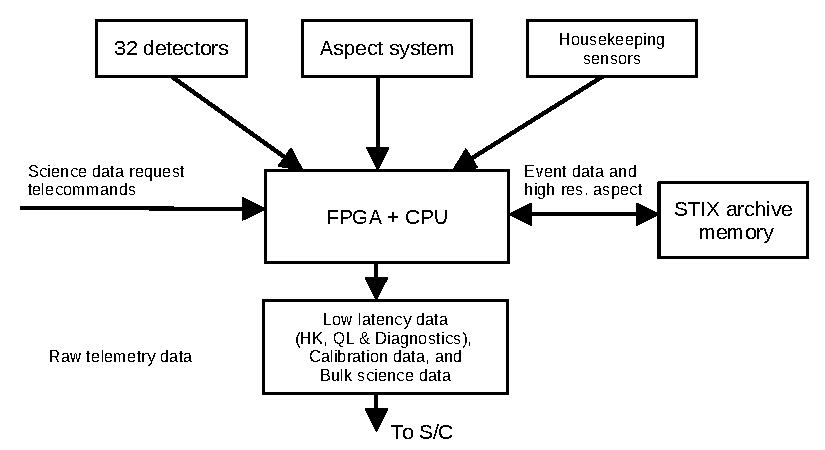
\includegraphics[width=0.8\linewidth]{figures/onboardDataFlow.pdf}
    \caption{STIX onboard data flow and data types.}
    \label{fig:stix_onbard_data_flow}
\end{figure}

STIX could process a maximum of 800,000 events per second (GOES X10 flares), which corresponds to  a data stream  of 20 MBits/sec. The event data needs to be reconciled to an average telemetry rate of 750 bits/sec.  This is done by an FPGA and a CPU located in the instrument Data Processing Unit (IDPU).  The FPGA is used for highly demanding tasks such as summing and sorting the event data stream into accumulators in the SDRAM.  Then application software running on the CPU processes the data in SDRAM 
in three parallel data paths by the flight software (FSW) running on the CPU: primary event processing, quick look processing and calibration data processing. 

For the primary event processing, the high-resolution signal amplitude values are first adjusted slightly by the FPGA to compensate for the current detector temperature, and then converted 
into one of 32 quasi-logarithmic detector-matched ‘science energy bins’ by the FPGA using a lookup table. Counts as a function of energy, detector ID and pixel number are accumulated in accumulators with a variable integration time that is a multiple of 0.1 second.  
The accumulation is truncated when a suitable number of counts have been reached or the accumulation time exceeds the pre-defined maximum value.

The contents of these accumulators are compressed and transferred to a rotating memory. 
Within a timescale of minutes, the ASW transfers the data from the rotating memory to a 16 Gigabyte flash memory, which is able to store several months of data.

Note that the processing to this point, done ‘blindly’ by the FPGA and FSW so that there is no data selection or statistically-significant loss of science–relevant information content. Data selections are done by the processor as  background tasks, based on  post facto uploaded requests via ground commands, originating from the STIX operations team.
There are two stages to the processing of the selected time/energy range by the instrument processor: the first step is selective averaging into science-relevant time and energy bins; The parameters are explicitly uploaded as part of user data requests.  The second stage is to  compress the selected data. The output of the compression algorithms is converted to telemetry packets and stored in the instrument telemetry buffer. 

The second data path is quick look processing.  Individual events are summed into a set of 16-bit accumulators after being corrected for temperature effect and converted to science energy channels. 
The accumulation time is fixed (can be adjusted by telecommand) with a default of 4 seconds. 
Corresponding triggers are also accumulated into 16 24-bit accumulators. The contents of these quick-look accumulators are used by the FSW for several purposes: flare identification, the determination of flare position and as input into spatially-averaged spectra and light curves for inclusion in the quick look data. The specifics of the averaging are defined by TC parameters, but the goals are to provide an overview of solar activity, and to monitor individual detector performance.
The purpose of the 3rd data path is to provide data for energy calibration. In this case individual events are accumulated with their temperature-corrected scaled A/D resolution but only during quiet times and with very long accumulation times (day). This provides detector-based
background spectra that include features from the calibration source that can be used on the
ground to establish and monitor the detector energy gain and resolution. To avoid
contamination of background spectra by periods of enhanced (but still low level) solar activity,
counts are only be accumulated if no other counts occurred in the preceding TC-specified
number of seconds.
The data directly read from STIX hardware can be divided into three categories. The first category is housekeeping data, which include voltage and current of power supplies, temperature sensor readouts; The second category is event data read from the 32 CdTe detectors, including the digitized photon amplitudes recorded by the 384 CdTe pixels detector, as well as the triggers. The third category is aspect system photo-diode readouts, which can be used to determine the pointing directions of STIX. 

 Aspect data is handled by a combination of the FPGA and FSW starting from the 1 kHz 12-bit
digitization of the output of the 4 aspect photodiodes. Low time resolution averaged aspect
data is included in HK telemetry. In addition, user TC requests can include selected intervals
with higher time resolution as part of the bulk science T/M. Details of the on-board aspect
data handling can be found in RD18. No on-board aspect interpretation is required for
instrument operation.
In addition to these STIX specific instrument functions, the IDPU provides the normal functions
of instrument level command interpretation and execution, commanding bias voltage levels in
response to ground commands or internally generated criteria, commanding attenuator state
changes, digitizing, monitoring and multiplexing instrument temperature sensor output, etc.
Both quick-look and science data are buffered internally so that although the rate of STIX-
generated data will be strongly dependent on solar activity, the data can be metered to the
spacecraft at a rate and cadence determined by the spacecraft requests.
The IDPU includes memories (ROM, RAM, and Flash) for data accumulation and software. It
interfaces to the Payload Data Management Unit, a housekeeping system, and other STIX
electronics (detector ASICs, aspect diodes readout, attenuator control, and power supplies).
By use of an autonomous state machine, it manages a rotating memory. The interfaces
between IDPU and the spacecraft are realized through a SpaceWire link (protocol
implemented in FPGA with additional external drivers/receivers).
STIX uses a robust algorithm to set a flare flag that includes information on the intensity,
spectrum and location of the event. This information will be used internally as input to the data
compression algorithms and sent to the s/c for optional transmission to other instruments for
use in choosing to observe modes or data selection.
Implementing the data flow in hardware, initial accumulation in the 64 MByte rotating memory
is done autonomously using an FPGA-based hardware state machine. The same FPGA
provides all necessary logic to interface the rotating memory to the main STIX processing unit.
The interface is organized in such a way that the data can be accumulated by the state
machine, while at the same time is available for access by the processing unit.
The architecture of STIX IDPU is presented in Figure 2-23. Communication with ASICs and
conversion of amplitude into 32 energy bins are performed in State Machines in Main (or
Redundant) IDPUs. Initial accumulation in the rotating memory (64MByte rotating memory) is
done autonomously using an FPGA-based hardware State Machine inside each of FPGAs.
FPGA provides all necessary logic to interface the rotating memory to the main STIX
processing unit implemented (as IP core) inside the same FPGA. The interface is organized
in such a way that the data can be accumulated by the rotating memory, while at the same
time is available for access by the processing unit. The total volume of the memory is 128
Mbytes, less than half of which is allocated for S/W operations. The rest of the memory can
be allocated to rotating memory, implying that the 64 MByte available for rotating memory is
a conservative estimate.
The LEON 3FT synthesized on Actel RTAX2000S/SL core is the baseline for the digital data
processing unit. It provides 20 MIPS of processing power. Since the State Machines internal
the CPU FPGA handle the time-critical tasks, the LEON3FT is primarily concerned with the
processing tasks mentioned in previous paragraphs.


More details descriptions of on-board data processing can be found in 
STIX telemetry can be classified in four categories: Housekeeping, Quick-look, Diagnostic
, and user requested Bulk Science (user-requested). HK and QL will be directed to the
 low Latency data store in Spacecraft Solid State Mass Memory (SSMM). 
For the most part, STIX data are organized by data content, with each major data content type
(e.g. x-ray imaging data, spatially-averaged x-ray data, HK data, etc.) associated with its own
packet types. While the format of each packet type is fixed, the relative frequency of each
packet type is dependent on solar activity and/or instrument mode.
Although the mix of packet types will vary, the 1-day average of HK and QL will respect the allocated rate of 4.3 Mbits/day (50 bps) each. The sum of all data types will respect the orbital average of 1.8 Gbits/orbit (700 bits/second for 30 days). STIX can make use of an onboard memory to load the SSMM at a rate compatible with spacecraft requirement.

\section{Data processing pipelines at STIX data center}



\subsection{Data link and data reception}
Telemetry generated by STIX are first be stored in the spacecraft solid state disk.
They are transmitted to ground data station when they are passes.  
After being received by the ground station of SOLAR Orbiter, it will be processed by ESA and stored in the EEDS database. ESA provides a web interface. The payload data must be created through the EEDS web page to create a data download request. After receiving the user's data request, EDDS displays the original payload data in the form of hex code and sends it to the stix data center server through the RSYNC protocol. Users can define the time interval of data request. Generally speaking, STIX server requests data from EDDS once a day. The data STIX obtains from EDDS is a HEX code with a time stamp, which is the same as the data sent by STIX to the spacecraft platform after being converted into binary data.
\subsection{STIX raw data processing pipeline}
\subsubsection{Raw data parsing}

include a decompression error map here
\subsubsection{Background monitoring}
Light curves measured during quiet periods of the sun are used for background estimation. Median values and of counts are computed and considered as the background in the selected time frame. They are stored in a database and used for flare identifications. 
\subsubsection{Flare identification}
Quick-look light curves in the energy range 4 to 10 keV are used for solar flare identification.  The flare identification procedure consists of  two steps:
\begin{itemize}
\item Light curve smoothing. In order to filter spikes from electronics and to reduce the amount of variation due to statistics and the onboard integer compression, light curves are smoothed by using the average filtering. The 
\item Flare identification. Local maximums are selected from smoothed light curves.  A local maximum is considered as a flare peak if the counts are exceeds 2 standard deviations above the background and the duration above the background is longer than 1 minute.  
\end{itemize}

For each of identified solar flares,   the  information such as start time, end time, counts, background subtracted counts is stored in the STIX flare database.   It is used for automatic creation of data requests for on-board archived data. 

\subsubsection{flare ID naming convention}
\subsubsection{Flare locations}
\subsection{Calibration data processing}

Ba134 radioactive sources with a total activity of about 4000 Bq are placed at the front of each detector. The total activity of the radioactive source is approximately 4000 Ba.
When the radioactive source decays, gamma rays are generated. These gamma rays can form peaks in the energy spectrum of the detector.
The corresponding energy is known, and the corresponding relationship between ADC and real energy can be calibrated through the position of the peak in the energy spectrum, that is, the calibration coefficient. The figure below is a typical Ba133 gamma-ray energy spectrum measured by STIX CdTe detector. There are three obvious peaks in the energy spectrum, and they correspond to three energies of 30 keV, 35 keV and 81 keV. There are many ways to determine the position of each peak, you can use the ECC method, or use the Gaussian function to fit the left part of the peak.

\subsubsection{Flare location using coarse flare data}
\subsubsection{Flare classification using GOES x-ray flux}
\subsubsection{FITS file creation}
\section{STIX data products}
\begin{itemize}
    \item Raw data.
    \item L1 data.
    \item L2 data
    
\end{itemize}

The latest level 1 FITS IO from Shane has been integrated into the data processing pipeline on pub023 server.

I have recreated fits products for all old telemetry data with the upgraded SW.

The L1 fits files  created by this pipeline have a different data level:  L1A ('A' here means  prerelease/alpha version).

The idea behind L1A data sets is to allow for quicker access to STIX data in the fits format instead of grabbing  data from plots or using JSON requests,

for operations,  debugging  etc.

The L1A data sets can be generated within a few minutes after the arrival of a new raw telemetry file.

The differences between L1A and L1 available in Shane's ftp include:

1.  Two different L1A data files may have duplicated data

2.  L1A data sets are still created for incomplete packets  (L1 checks for data completeness)

3.  SPICE kernel data for telemetry files always arrives  after one or two days later.
    So  there may be a sub-second difference between the UTC time in fits files (same to times on web pages)

   and the real time.

    Shane's formal L1 release can avoid this issue if they are produced on a later date.

4. L1A contains housekeeping data




The Level0 archive contains TM which has been parsed or decommuated into readable structures but no additional external information is include:

times are not converted to UTC
no calibration or conversions applied
for STIX we need to decide if we decompress / combine X-ray L0 the count/trigger data at this stage or in the next level L1

copy manual,
tree like, 
json formats
name, raw value, eng value, children
look-up table, to know description

estimate mongodb benchmark
Mongodb benchmark,
key value, index, performance



\begin{table}
\centering
\caption{Level 1 data products}
\begin{tabular}{llll}
Category & Type   &  Naming convention  & Remarks   \\ \hline
 Housekeeping & hk\_mini  &  & Houskeeping in BOOT mode   \\
 & hk\_maxi  &  & houskeeping data in NOMINAL   \\
 Quick-look &  light curves &  & Quicklook lightcurves \\
  &  variance &  & variance \\
  &  spectra &  &  \\
  &  background monitor &  &  \\
    &  flare location &  &  \\
 Calibration data &   &  &  \\
\end{tabular}
\end{table}

\section{Data request procedure}
created of data requests
manuall checked
\textbf{  data request naming convention  yyddmm00  to yyddmm 11 }


\section{Flare processing}

\section{Database}
\subsection{Raw data packet database } 
\subsection{Configuration database}

\section{Online data visualization tools}
\subsection{Quick-look light curve}
\subsection{Science data quick analysis}
\subsubsection{Calibration data}
\begin{figure}
    \centering
    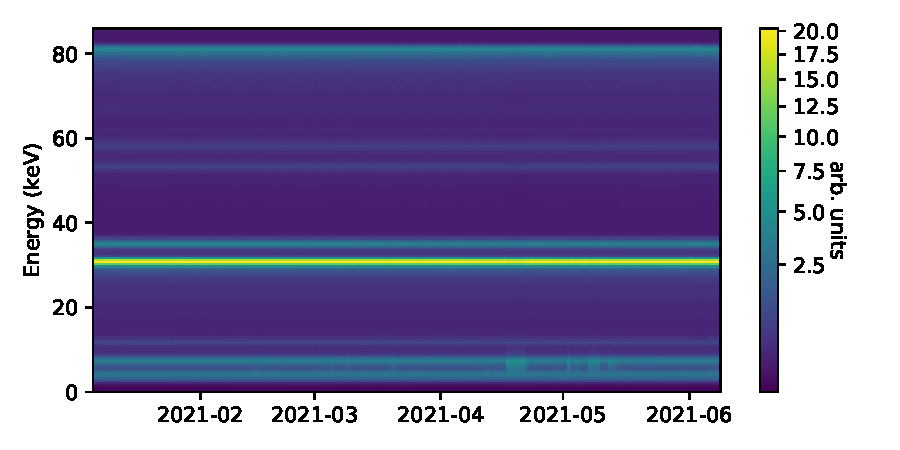
\includegraphics[width=0.8\linewidth]{figures/calibrationSpectrogram.pdf}
    \caption{Caption}
    \label{fig:calibrationSpectrum}
\end{figure}
\begin{figure}
    \centering
    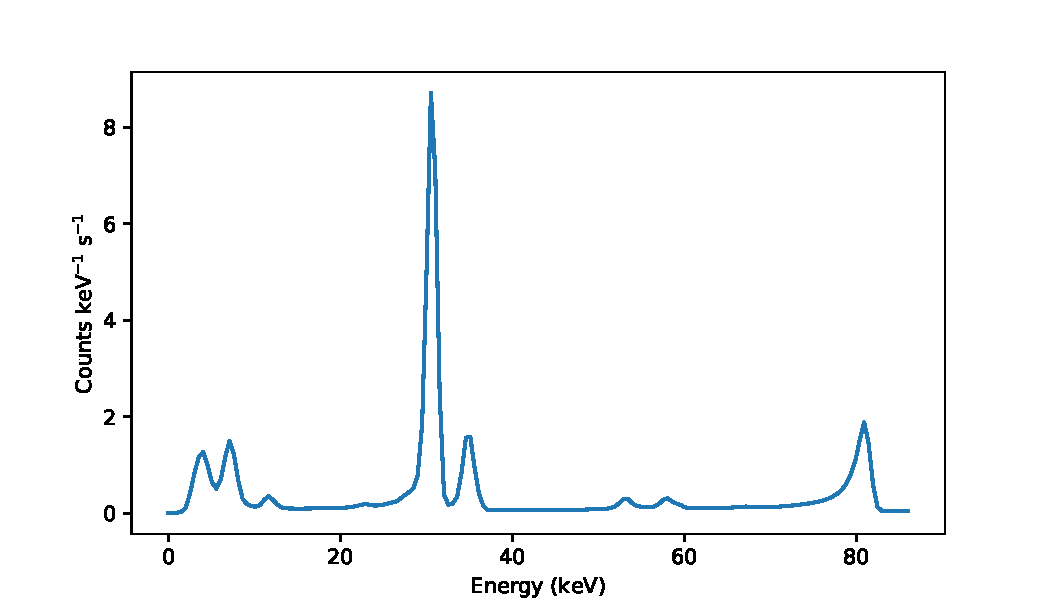
\includegraphics[width=0.8\linewidth]{figures/calibrationSpectrum.pdf}
    \caption{Spectrogram of STIX calibration spectra}
    \label{fig:calibrationSpectrogram}
\end{figure}

calibration data products
https://fermi.gsfc.nasa.gov/ssc/data/access/gbm/
\subsubsection{Solar Orbiter orbit viewer}


When a new data file from the platform is received at the PPDC,
it triggers an autonomous start of the dedicated program that decodes and
interprets its contents. The binary data contain the spacecraft location, attitude, speed, and GPS timestamps with increments every half second. The GPS timestamps are converted into Unix-timestamps, where the leap seconds are also considered. After processing, the platform data are written to the ROOT format files. The data start and stop time, data processing time, input filename and ID of the output file of each processing are recorded in a dedicated database table.
SPICE kernel

Updated once per day.

At the center of the Sun.
It is worth mentioning that has to corrected for.
This can be done by using the web tool provided at the auxiliary data center at


\section{Data access and APIs}
\section{Future work}
\section{Conclusions}




% WARNING
%-------------------------------------------------------------------
% Please note that we have included the references to the file aa.dem in
% order to compile it, but we ask you to:
%
% - use BibTeX with the regular commands:
%   \bibliographystyle{aa} % style aa.bst
%   \bibliography{Yourfile} % your references Yourfile.bib
%
% - join the .bib files when you upload your source files
%-------------------------------------------------------------------

\bibliographystyle{aa}
\bibliography{citations}

\end{document}
